%https://tex.stackexchange.com/questions/344838/3d-surface-plot-with-color-to-represent-4th-dimension

\documentclass[border=5pt]{standalone}
\usepackage{pgfplots}
\pgfplotsset{compat = newest}
 
\begin{document}
    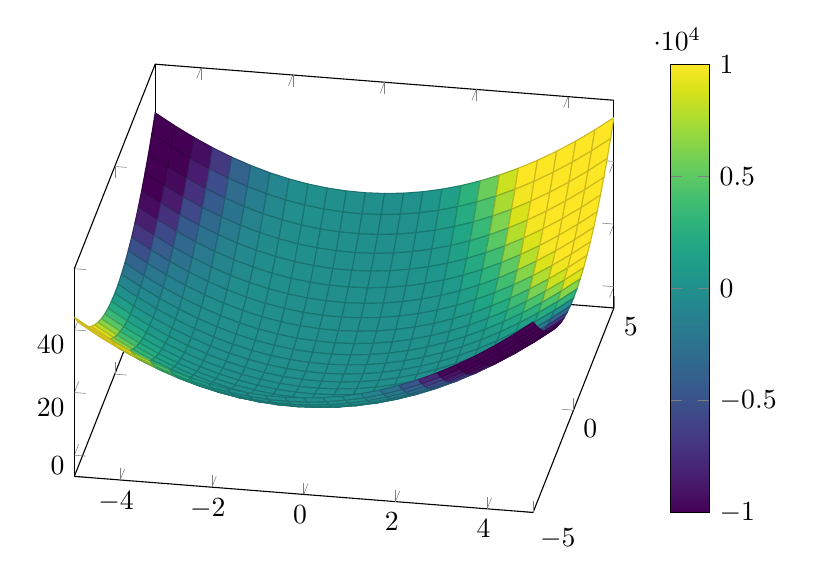
\begin{tikzpicture}[
        declare function = {%
            q(\x) = \x - 1;%
            Z(\x,\y) = \x^2 + \y^2 + q(\x);%
            w(\x,\y,\z) = \x^2 * (3 + 2*\x)*(1+\x*\y)*(1+\x*\z)/(1+\x^2);%
        }%
    ]%
        \begin{axis}[
            colormap/viridis,
            colorbar,
            view={10}{45},
            point meta min=-1e4,
            point meta max=+1e4,
        ]
            \addplot3 [
                surf,
                point meta={w(x,y,z)}
            ] {Z(x,y)};
        \end{axis}
    \end{tikzpicture}
\end{document}